\newpage
\section{Part I - Mathmatical modeling}

In this chapter we construct a mathematical model, defining the helicopters three axes; pitch, elevation and travel. 

\begin{figure}[!htb]
    \centering
    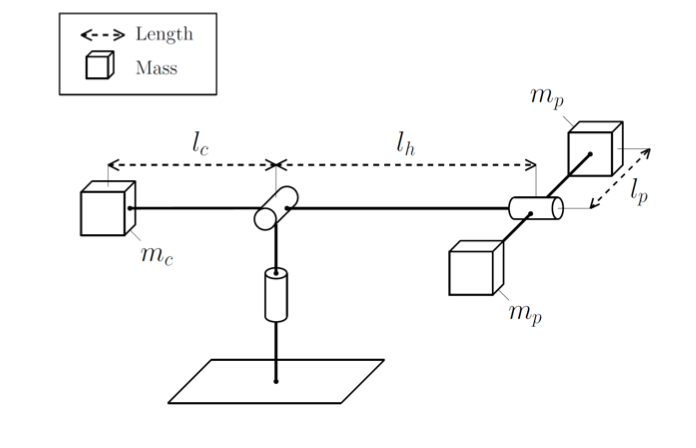
\includegraphics[scale=0.8]{images/model}
    \caption{Model dimensions}
    \label{poles}
\end{figure}

\begin{figure}[!htb]
    \centering
    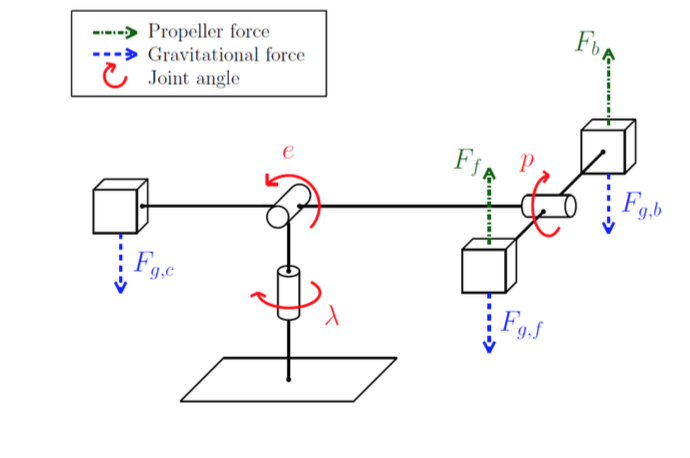
\includegraphics[scale=0.8]{images/model2}
    \caption{Model momentum and forces}
    \label{poles}
\end{figure}
\newpage
A relationship between the motor force and the motor voltage is given by:
\begin{equation}\label{eq:force_f}
    F_f =K_fV_f   
\end{equation}
\begin{equation}\label{eq:force_b}
    F_b  =K_fV_b  
\end{equation}

Equations (\ref{eq:force_f}) and (\ref{eq:force_b}) show that the relationship between motor force and motor voltage is proportional to a constant $K_f$. The equations describing the plant are then transformed into a state-space model.


%-------------------------------------
           % Derivation of the model%
%-------------------------------------

\subsection{Problem 1 - Derivation of the mathematical model}
Newton's second law gives a relationship between the net external torque and the angular acceleration, this relationship will be used to derivate the mathmatical model for pitch, elvation and travel.


%-------------------------------------
               % Pitch%
%-------------------------------------
\subsubsection{Derivation of pitch}
 Sum of torque on the pitch axis is given as: $ \Sigma{\tau}= J_p \ddot{P} $. 
  

Further, the magnitude of torque is given by $ \tau=r\times F = |r||F| \sin(\theta) $,
where $ \theta $ is the angle between the force vector and the lever arm vector. We consider $\theta=90^{\circ}$ to derive the following pitch equation:

%\begin{equation} 
\begin{align} 
\Sigma{\tau}_{\tau} &=  rF \nonumber \\ 
 &=  (F_f-F_b)l_p \nonumber\\
 &=K_f l_p (V_f-V_b)&&\text{(substituting \ref{eq:force_f} and \ref{eq:force_b})} &  \nonumber\\
 &= K_f l_p V_d &&\text{($ V_d = V_f - V_b$)} \nonumber \\
 &=L_1V_d = J_p \ddot{P} &&\text{(Where $L_1=K_f l_p$ is a constant)} \nonumber\\\nonumber
 \\ 
 J_p \ddot{P}&=L_1V_d \label{eq:pitch}
\end{align}
%\end{equation}



%-------------------------------------
            %Elevation%
%-------------------------------------
\subsubsection{Derivation of elevation}
The forces acting on the elevation axis are $F_{g,c}$ and $F_f + F_B$ giving the vertical thrust 
The sum of $F_f + F_B$ determines the vertical thrust. 
On the elevation axis both $F_{g,c}$ and the sum of the two forces $F_f$ and $F_b$ giving the thrust vertical to the x axis. 

\begin{align} 
\Sigma{\tau}_{e} &=  rF \nonumber\\ 
 &= {{m_c}g{l_c}\cos (e) - 2{m_p}g{l_h}\cos (e) + ({K_f}{V_f} + {K_f}{V_b}){l_h}\cos (p)} \nonumber\\ 
 &= ({m_c}{l_c} - 2{m_p}{l_h})g\cos (e) + {l_h}{K_f}{V_s}\cos (p) = {J_e}\ddot e\g 
 &&\text{(substituting \ref{eq:force_f} and \ref{eq:force_b})} \nonumber\\ 
 &= L_2\cos(e)+ L_3 \cos(p)v_s = J_e\ddot{e}  &&\text{( $ 
{L_2} = ({m_c}{l_c} - 2{m_p}{l_h})g$, $L_3=l_h K_f$)} \nonumber \\
\nonumber\\
 J_e\ddot{e}&= L_2\cos(e)+ L_3 \cos(p)v_s \label{eq:elevation}
\end{align}


%-------------------------------------
            %Travel%
%-------------------------------------

\subsubsection{Derivation of travel axis}
There are two forces acting on the travel axis, thrust force and rotor's torque has an impact on the elevation axis

\begin{align} 
\Sigma{\tau}_{\lambda} &=  rF \nonumber\\ 
 &= L_4 V_s \cos(e) \sin(p) =J_\lambda \ddot{\lambda} && \text{(Where $L_4=L_3=l_h K_f$)} \nonumber\\
 \nonumber \\
J_\lambda \ddot{\lambda}&=L_4V_s\cos(e)\sin(p) \label{eq:travel}
\end{align}

 
